\documentclass{article}
\usepackage{graphicx}
\usepackage{moreverb}
\begin{document}

\title{Predicting the performance behavior of \\ Stencil applications with static code analyses}
\author{Tan Nguyen}

\maketitle
\date

\section{Introduction}
The ability to quickly characterize the performance behavior of an application on various processor architectures is one of the most important requirements for exascale design.
Indeed, the huge hardware design space together with the large number of applications of interest prevent dynamic approaches from working effectively.
This report shows extensions to ExaSAT \cite{exasat,exasat1}, a performance prediction tool that can instantly evaluate program source code on many hardware configurations, to assist exascale design efforts.
ExaSAT consists of two components: an analyzer that extracts knowledge about the application and a performance model that predicts the application performance using adjustable hardware parameters. 
While the existing set of hardware parameters is relatively complete, the code analysis component is not sophisticated enough to capture useful aspects of a practical program.

We supplement ExaSAT with deeper analyses to enhance the accuracy of our performance evaluation.
The analyses presented in this report focus on stencil-based applications, which are anticipated to account for a majority of workload on future exascale systems.
Such applications approximate solutions of partial differential equations by iteratively sweeping an operator called {\em stencil} over discrete meshes. 
Stencil operators update each data element using values of surrounding neighbors.
Although stencil operators written in a mathematical representation can be easily recognized, automatically extracting stencil code from practical programs is challenging due to various programming styles used by the programmer for array references.
In addition, the representation and usage of multi-dimensional arrays in different languages may differ.
We enhanced the analyses of Exasat, enabling this tool to support commonly used array reference styles.
The tool also supports applications written in C, Fortran, and the mix of these 2 languages.

\section{ExaSAT in a nutshell}
In this section we briefly summarize the ExaSAT framework, which consists of 2 main components: a code analyzer that studies application characteristics and a performance model that takes arguments for system parameters and the application information extracted by the code analyzer to predict the performance.

\subsection{Static code analyzer}
The code analyzer of ExaSAT is built on top of the ROSE compiler framework.
ROSE consists of frontends, a midend, and backends.
For every source file written in a particular language, there is a frontend that parses the source code into an intermediate representation (IR) called ROSE AST (abstract syntax tree).
The code analyzer extends the midend to analyze the IR generated by ROSE.
ExaSAT currently does not use backends to unparse the IR to source code since code transformation is not an objective of ExaSAT. 
The code analyzer generates useful information of the input code such as function calls, loops, floating point operations, scalars, and array access patterns, etc.
This information is stored in an XML file using a higher level description that can be read and manipulated by the programmer.

\subsection{Performance model}
The existing performance model of ExaSAT focuses in 2 categories: computation capability and memory system. 
Not only can Exasat estimate the application running time, it evaluates the asymptotic performance by calculating the ability of the memory system in supplying data for computations. 
For floating point operation, ExaSAT allows the programmer to provide the costs of different types of operations. 
For example, divides and transcendentals are often more costly than add and multiply.
Since most computations requires data to be fetched from main memory to registers, ExaSAT takes the memory bandwidth and cache/register size into consideration.


\section{Array access analysis}
On modern processor/node architectures, accessing memory is increasingly costly due to a substantial reduction in the amount of memory per core and the prominence of NUMA architecture.
The problem is more exarcebated by the prevalence of stencil kernels in production codes, placing high bandwidth demands on the memory systems.
As a result, our analyses focus more on memory access operations than on floating point ones.
Stencil operations on 1-dimensional arrays can be easily recognized in a well formulated form as shown in Eq. \ref{eq:stencil}.
However, practical applications often make use of multi-dimensional arrays and various styles to reference an array, challenging any attempts to recognize stencil operations automatically.

\begin{equation}
U'[i] = c * \sum^{k \in S} c_{k} * U[i \underline{+} k] 
\label{eq:stencil}
\end{equation}

where, U and U' are array names (which can be identical in some solvers), the array index {\em i} varies, S is a set of small integers, and {\em $c_{k}$} is a coefficient associated with k.

In this section we outline common fashions that the programmer often uses to access multi-dimensional arrays.
In addition, we present high level algorithms to analyze codes written in these styles.
More formal analyses will be presented in the next section.


\subsection{Example}
To illustrate our analyses, we use the classical 7-point stencil kernel, which approximates the solution for Laplace's equation ($Lu \equiv \nabla \cdot . \nabla u = 0$) in 3 dimensions.
The following code snippet shows a Matlab implementation of this solve0.
The stencil operator is characterized by a 3x3x3 matrix, in which 6 nearest neighbors have weight 1 while the others including the central element have weight 0.
For each time step, the kernel sweeps this operator over the discrete domain of the solution.

\begin{figure}[htp]
\begin{boxedverbatim}
    for iter= 1:nIters
      Un[:,:,:] = (U[:,:,:] .* M)/6.0 
      swap(U, Un)
    end
\end{boxedverbatim}
\caption{A Matlab implementation of the 7-point stencil kernel. A 3x3x3 matrix representing the Laplace operator is swept over matrix U, multiplied with submatrices of U to update the central data elements.}
\label{7pointstencil}
\end{figure}

\subsection{Fortran-style array referencing}
Fortran supports multi-dimensional arrays.
To declare an array and allocate its memory the Fortran programmer specifies rank, shape, and extent.
Rank is the number of dimensions of an array; shape is the number of elements in each dimension; every dimension has an extent, which is the range of its index.

There are three schemes to explicitly reference a Fortran multi-dimensional array, as follows.

\begin{enumerate}
\item Indexing: subscripts of an array reference expression refer to an individual element of the array, e.g. U(i,j,k), where U is array name and i, j, and k are subscripts. 
\item Subarray: a subscript with the {\em :} operator refers to a range of elements, e.g. U(1:10,1,1) refers to 10 elements from U(1,1,1) to U(10,1,1).  
\item Whole array: an array name without any subscript, e.g. U, refers to the entire array.
\end{enumerate}

For the first and second schemes outlined above, the ROSE's frontend represents each array reference expression with a special data structure comprising an IR node representing the array variable reference and multiple IR nodes representing subscript expressions.
For the third case, the frontend employs a generic variable reference node to represent a whole array reference expression.
However, this IR node is associated with an array type node, distinguishing it from the other kinds of variable references. 
In all 3 cases, ExaSAT can easily detect array reference expressions due to such distinct representations.
If a reference expression is written in the stencil form governed by Eq.~\ref{eq:stencil}, the constant offset (i.e. $\underline{+} k$) is analyzed independently within each individual dimension. 
For example, the statement to update Un in Fig.\ref{7pointstencil} can be written in Fortran as follows:
{\em Un(i,j,k) =  (U(i,j,k-1) + U(i,j,k+1) + U(i,j-1,k) + U(i,j+1,k) + U(i-1,j,k) + U(i+1,j,k))/6.0}.
Exasat will generate a series of offsets associated with each array (i.e. Un and U).

\subsection{C-style array referencing}
Like Fortran, C also supports multi-dimensional arrays.
However, the C programmer specifies only rank and shape of an array.
The extent of each array dimension always begins with 0.

Unlike in Fortran, indexing is the only way to reference a C array.
For example, U[k][j][i] refers to the element that has indices k, j, and i.
The statement to update Un in Fig.\ref{7pointstencil} can be written in C as follows: {\em Un[k][j][i] =  (U[k-1][j][i] + U[k+1][j][i] + U[k][j-1][i] + U[k][j+1][i] + U[k][j][i-1] + U[k][j][i+1])/6.0}.

There is another difference between C and Fortran arrays.
That is, C treats a multi-dimensional array as an array of arrays, resulting in different representations for array references at the compiler level.
With respect to the example above, ROSE's frontend employs 3 array reference expression nodes for a single array reference U[k][j][i].
In addition, these nodes are nested as follows.
At the top level, we have U[k][j] node and an expression node representing the subscript i.
Under U[k][j] is U[k] going along with a node representing the subscript j.
Finally, U[k] contains U and the associated k subscript.
To handle this array of arrays representation, ExaSAT recursively looks up array reference expression nodes until no more is found.
For each node, ExaSAT extracts information of the corresponding index.
Once all the indicies are found, ExaSAT determines whether the array reference is in stencil form using the same method as with Fortran arrays.

\subsection{Flattened array indexing}
No matter what language is used, the programmer can always implement a multi-dimensional array based on a one-dimensional array.
Indeed, the programmer can manually embed a high-dimensional data layout in a flat array and establish a one-to-one mapping between the indices of the 2 arrays. 
The memory distance to increment the index in a high-order dimension is called a {\em stride}. 
For example, the array reference expression U[k+1][j][i]  can be mapped to U[(k+1)*kStride + j*jStride+ i], where kStride and jStride are {\em strides} for the third and second dimensions respectively.

When an array has been flattened, subsequent array accesses are very difficult to analyze due to complicated subscript expressions.
Fortunately, the performance model of ExaSAT is interested in memory references residing in loops only.
In addition, loop iterator variables are used in the subscript expression. 
These common facts suggest that strides go along with loop dependent variables.
Thus, one can find out the stride for each array dimension among variable references in a flat array subscript expression, assuming that no stride variable reference is calculated based on another.
Once we can reason about strides, corresponding offsets can also be found since they go with strides instead of with loop dependent variables. 

\subsection{Pointer dereferencing}
Pointer support is essential in any language. 
In Fortran (F90 and later), a pointer has to have a specific rank.
The Fortran programmer does not need to dereference a pointer to reference an array.
Instead, he/she uses pointer as an alias.



\begin{figure}[htp]
\begin{boxedverbatim}
 for (int iter=1; iter<=nIters; iter++){
   for (int k=1; k< nz-1; k++) {
     for (int j=1; j< ny-1; j++) {
       double *Un0;
       Un0 = &Un[k][j][0];
       double *up  = &U[k-1][j][0];
       double *down = &U[k+1][j][0];
       double *north = &U[k][j-1][0];
       double *south = &U[k][j+1][0];
       double *west = &U[k][j][-1];
       double *east = &U[k][j][1];
       for (i = 1; i < nx-1; i++){
         *(Un0+i) = (*(up+i) + *(down+i) + *(north+i) + \ 
         *(south+i) + *(west+i) + *(east+i))/6.0;
       }
     }
   }
 }
\end{boxedverbatim}
\caption{A C implementation of the 7-point stencil kernel using pointer dereferencing}
\label{7pointstencilPtr}
\end{figure}


The problem is more interesting with the C language.
In C, whether an array has one or multiple dimensions the programmer can access its data elements using a pointer and an offset. 
For example, *(ptr+i) refers to the i'th element couting from the first element pointed by pointer {\em ptr}, where * is the pointer dereference operator. 
We can access different elements of an array by varying the value of the pointer, or the offset, or both.
Fig.~\ref{7pointstencilPtr} shows a C implementation of the 7-point stencil kernel which uses pointer to access data element of U and Un arrays.
Tracking the memory address pointed by a C pointer is a challenging task.
However, there are some special cases where we can analyze such information.
For example, when {\em ptr} does not change its value throughout the enclosing loop and the offset {\em i} is a loop dependent variable, we can simply analyze the memory address pointed by the pointer before the execution of the loop.
Another simple case is that the offset is fixed (or there is no offset), and the value of the pointer is incremented/decremented by a constant factor of a loop dependent variable. We then can find the correlation between the variations of the pointer and the loop dependent variable to figure out how data elements of an array are referenced. 

\section{Formal Analyses}
In the previous section we presented simple analyses to extract memory access information from the source code.
In this section we formalize those analyses with dataflow and interprocedural analyses so that we can capture those cases in a general context where branches, loops, function calls, and lexcical scopes are present.


\subsection{Dataflow analysis}
TBW

\subsection{Interprocedural analysis}
TBW

\section{Experimental validation}
In this section we employ the code analyzer and the performance model of ExaSAT to study the performance behavior of two applications on various hardware architectures.
The first application is a contrived program, which approximates the solution of Laplace's equation in 3 dimensions using a 7-point stencil scheme.
The other application is widely known as HPGMG, a benchmark based on geometric multigrid.
This benchmark is a multigrid solver for Helmholtz's equation in 3 dimensions.

We conduct experiments on 3 node architectures: Cray XE6 (2x 12-core AMD's Magny-Cours processors connecting with HyperTransport links), 2x 8-core Intel's Sandy Bridge processors connecting with QPI links (SNB), and 2x 12-core Ivy Bridge connecting with QPI links (IVB).
% and Knights Corner (KNC) (61 in-order, pentium4-like cores connecting to a dual ring bus).
Cray XE6 and Intel IVB are respectively available on Hopper and Edison at NERSC while SNB is provided by Stampede at TACC.

For each node architecture, we collect hardware information, including memory bandwidth and peak computing rates (floating point operations).  
Using such information and other system parameters such as caching policies, we can predict the performance of different applications on various problem sizes.
We also collect memory profiling information to further validate the performance model, as well have to have deeper insights on the application behavior. 
We use PAPI, an instruction level profiling tool that counts hardware events such as the number of floating operations and L3 cache misses.
The L3 cache miss information can be used to calculate the amount of data transfer from DRAM to this lowest level cache.

We study various application problem sizes classified into 2 categories.
One fits in DRAM and the other fits entirely in L3 cache.
While the latter does not usually happen in practical applications, a similar situation is when a part of the problem can remain in L3 through multiple loops or multiple iterations within a loop before it needs to be copied back to DRAM.
Multigrid is an example, where grids at a coarse level may fit well in L3 cache.

\subsection{Calibration}
To measure memory bandwidth, we used the stream triad benchmark ($a[:] = b[:] + c[:] * scalar$).
We ran this benchmark on all available processor cores of a compute node.
We noticed that all node architectures employ a NUMA design, where the data bandwidth to local DRAM is much higher than to remote DRAMs.
As a result, we pinned threads to cores and used the first-touch memory placement to take advantage of data locality.
On Hopper and Edison, we can pin threads to cores using the command flag {\em -cc none} or {\em -cc numa}. 
On Stampede, we used the environment variable {\em KMP\_AFFINITY} to bind threads to cores.
We used Intel compiler in all experiments.
One can also use GNU compiler and the {\em GOMP\_CPU\_AFFINITY} variable as an alternative.

For peak GFLOPS/s performance, we use the HPL benchmark, which factors a matrix into lower and upper triangular matrix components.
The main kernel of this application is the level 3 BLAS routine AKA {\em dgemm}.
HPL is implemented on MPI.
Thus, its performance is not affected by NUMA effects.
We only use the peak GFLOP/S information to show that the applications that we study are memory bound.
This information does not contribute to the performance prediction of the 2 applications used in this paper.
Indeed, the computation time can be hidden by the vertical data transfer from DRAM to cache.


\subsection{7-point stencil}

\subsection{XML description}
Figure~\ref{7pointstencilOutput} shows the generated XML description of the 7-point stencil kernel presented ealier in Fig.~\ref{7pointstencilPtr}.
Using the XML description, one can recognize the memory access pattern of the kernel by looking at the offsets  and the access type (read/write/readwrite) of array references to U and Un.
The performance model of Exasat uses this information to reason about the data working set of the stencil kernel and the amount of data needs to be moved across the memory hierarchy.



\begin{figure}[htp]
\begin{boxedverbatim}
<loop line="166" lvar="k" lb="1" ub="nz-1" stride="1" adds="0" mults="0">
<loop line="167" lvar="j" lb="1" ub="ny-1" stride="1" adds="0" mults="0">
<loop line="177" lvar="i" lb="1" ub="nx-1" stride="1" adds="5" mults="1">
<array name="U" component="" type="double" access="readonly">
<access offset="(-1 ,0 ,0 )" lvar="(i, j, k)" reads="1" writes="0"/>
<access offset="(0 ,1 ,0 )" lvar="(i, j, k)" reads="1" writes="0"/>
<access offset="(0 ,0 ,0 )" lvar="(i, j, k)" reads="1" writes="0"/>
<access offset="(0 ,0 ,1 )" lvar="(i, j, k)" reads="1" writes="0"/>
<access offset="(0 ,0 ,-1 )" lvar="(i, j, k)" reads="1" writes="0"/>
<access offset="(0 ,-1 ,0 )" lvar="(i, j, k)" reads="1" writes="0"/>
<access offset="(1 ,0 ,0 )" lvar="(i, j, k)" reads="1" writes="0"/>
</array>
<array name="Un" component="" type="double" access="writeonly">
<access offset="(0 ,0 ,0 )" lvar="(i, j, k)" reads="0" writes="1"/>
</array>
</loop>
</loop>
</loop>
\end{boxedverbatim}
\caption{The XML description of the stencil kernel (after simplified), which contains 3 loop nests. The innest loop has 7 references to U and 1 reference to Un.}
\label{7pointstencilOutput}
\end{figure}

\subsubsection{Predicting the performance}
Here are different scenarios that the performance model can imply from the XML description.

\begin{enumerate}
\item An ideal data working set of the 7-point stencil kernel consists of 3 planes of U and no plane of Un.
For this ideal case, Un will be written to DRAM in streams, thus there is no need to maintain a copy of Un in cache.
Since the 3 planes of a working set are consecutive in the z dimension, an update to a plane of Un requires only one plane of U to be fetched from DRAM (the other 2 planes are already in cache).
Thus, the total number of planes transfered between DRAM and cache for the computation of a plane is 2 (1 read and 1 write).
In this report, we do not delve into this scenario since most processors do not support streaming write (including the 3 achitectures we use in this paper).
In the future, we will explore the effects of streaming write on Intel's MIC architecture which support this capanbility.

\item Since most processors do not support streaming write, a plane of Un has to be maintained in cache to avoid unoptimized writes to DRAM. Thus, the data working set consists of 4 planes (3 of U and 1 of Un).
As a result, the number of planes needs to be moved for a plane update is 3 (i.e. 2 reads and 1 write) instead of 2. 
We will refer to this case as {\em cached}.

\item If the programmer does not block for cache, a plane can be too big to fit in cache.
In this case, 5 planes (4 reads and 1 write) have to be moved for a plane update since we do not have enough space in cache to keep old data.
We refer to this case as {\em uncached}.
\item If the programmer blocks for cache but incorrectly calculate the data working set, a part of this set may be overwritten or spilled to DRAM.
With a LRU eviction policy, a plane of U may be overwritten if we don't have enough space in cache.
Thus, the number of planes transfered between cache and DRAM can be 4.
\item If the problem size is small enough to fit entirely in L3 cache, there is no need to fetch data from DRAM.
The new result of Un, however, needs to be written back to DRAM.
Thus, we only need to move 1 plane in this situation.
We refer to this case as {\em L3}.
\end{enumerate}


To verify the performance analysis above, we collect the number of L3 misses to calculate the amount of data needs to be copied to L3 cache per plane update.
Figure~\ref{l3misses_7point} shows the number of reads/writes from/to DRAM per plane update as the problem size increases.
With N=96, the total amount of data of the 2 arrays U and Un is $2* 96^3 * 8$ = 13.5 MB, which fits in L3.
As predicted, the number of reads is almost 0 and the number of writes is 1. 
With N=128, L3 has space to store only the read only array.
Thus, the number of reads is 1 and the number of writes is 1.
With N=128, 256, and 384 we have the normal case when arrays have to be stored in DRAM and L3 has enough space to cache the data working set.
Thus, the number of reads is 2 and the number of writes is 1.
With N=512, the amount of data has to be cached in L3 of a NUMA domain is 6 (cores) * 512 * (512/6) * 8 * 4 (planes) = 8 MB, which is larger than L3 capacity of the domain.
Thus, one plane is overwritten. This is the reason why the number of read planes increased to 3.
Similarly, with N=768 2 planes have to overwritten and the number of read planes increased to 4.


\begin{figure}[htp]
\centering
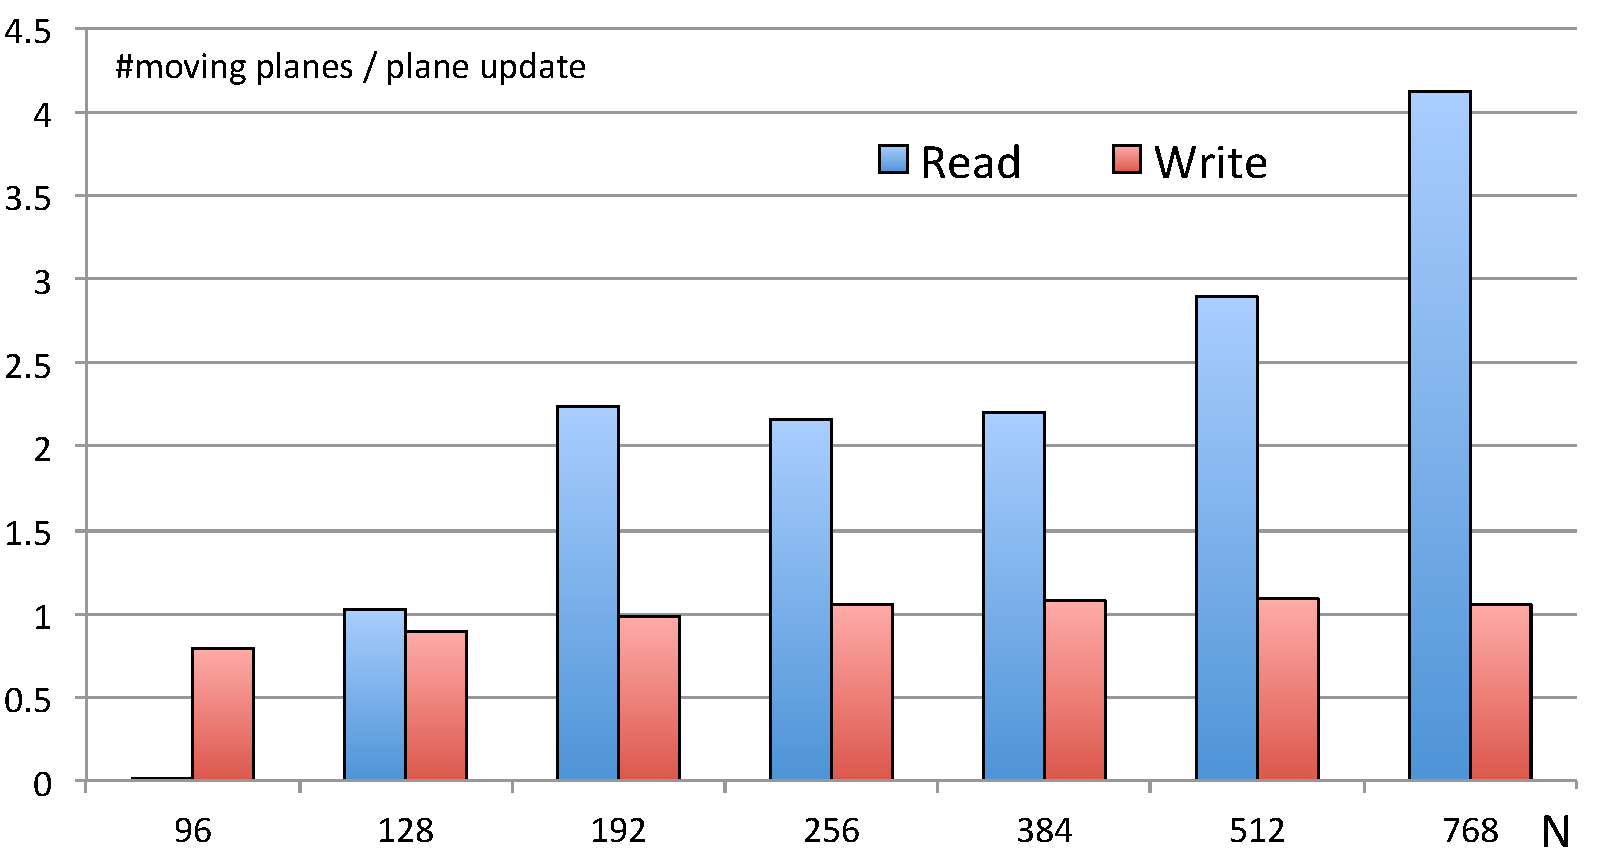
\includegraphics[width=0.99\textwidth]{l3misses_7point}
\caption{The number of reads and writes needed per point update on 1 single compute node of Hopper. These numbers are calculated based on the number of L3 cache missed, DRAM bandwidth, and the execution time.}
\label{l3misses_7point}
\end{figure}


We then evaluated the performance of 7-point stencil and compared with the predicted performance.
Since we measured the total performance (in GFLOPS/s), we included the inter-process communication.
We increased the problem size and selected 3 points corresponding to 3 cache behaviors presented above: {\em cached}, {\em uncached}, and {\em L3}.
Figure~\ref{jacobi_dram} shows the predicted and actual performance in GFLOPS/s of this application on 3 different processor architectures. 
It can be seen that the performance difference between the predicted and the measured results is consistent on all architectures (AMD Magny-Cours, Intel's Sandy Bridge and Ivy Bridge).
We found that our prediction was almost accurate with large problem size ({\em uncached}).
The accuracy reduced when the problem size decreased.
This is due to the increase in the communication overheads.


\begin{figure}[htp]
\centering
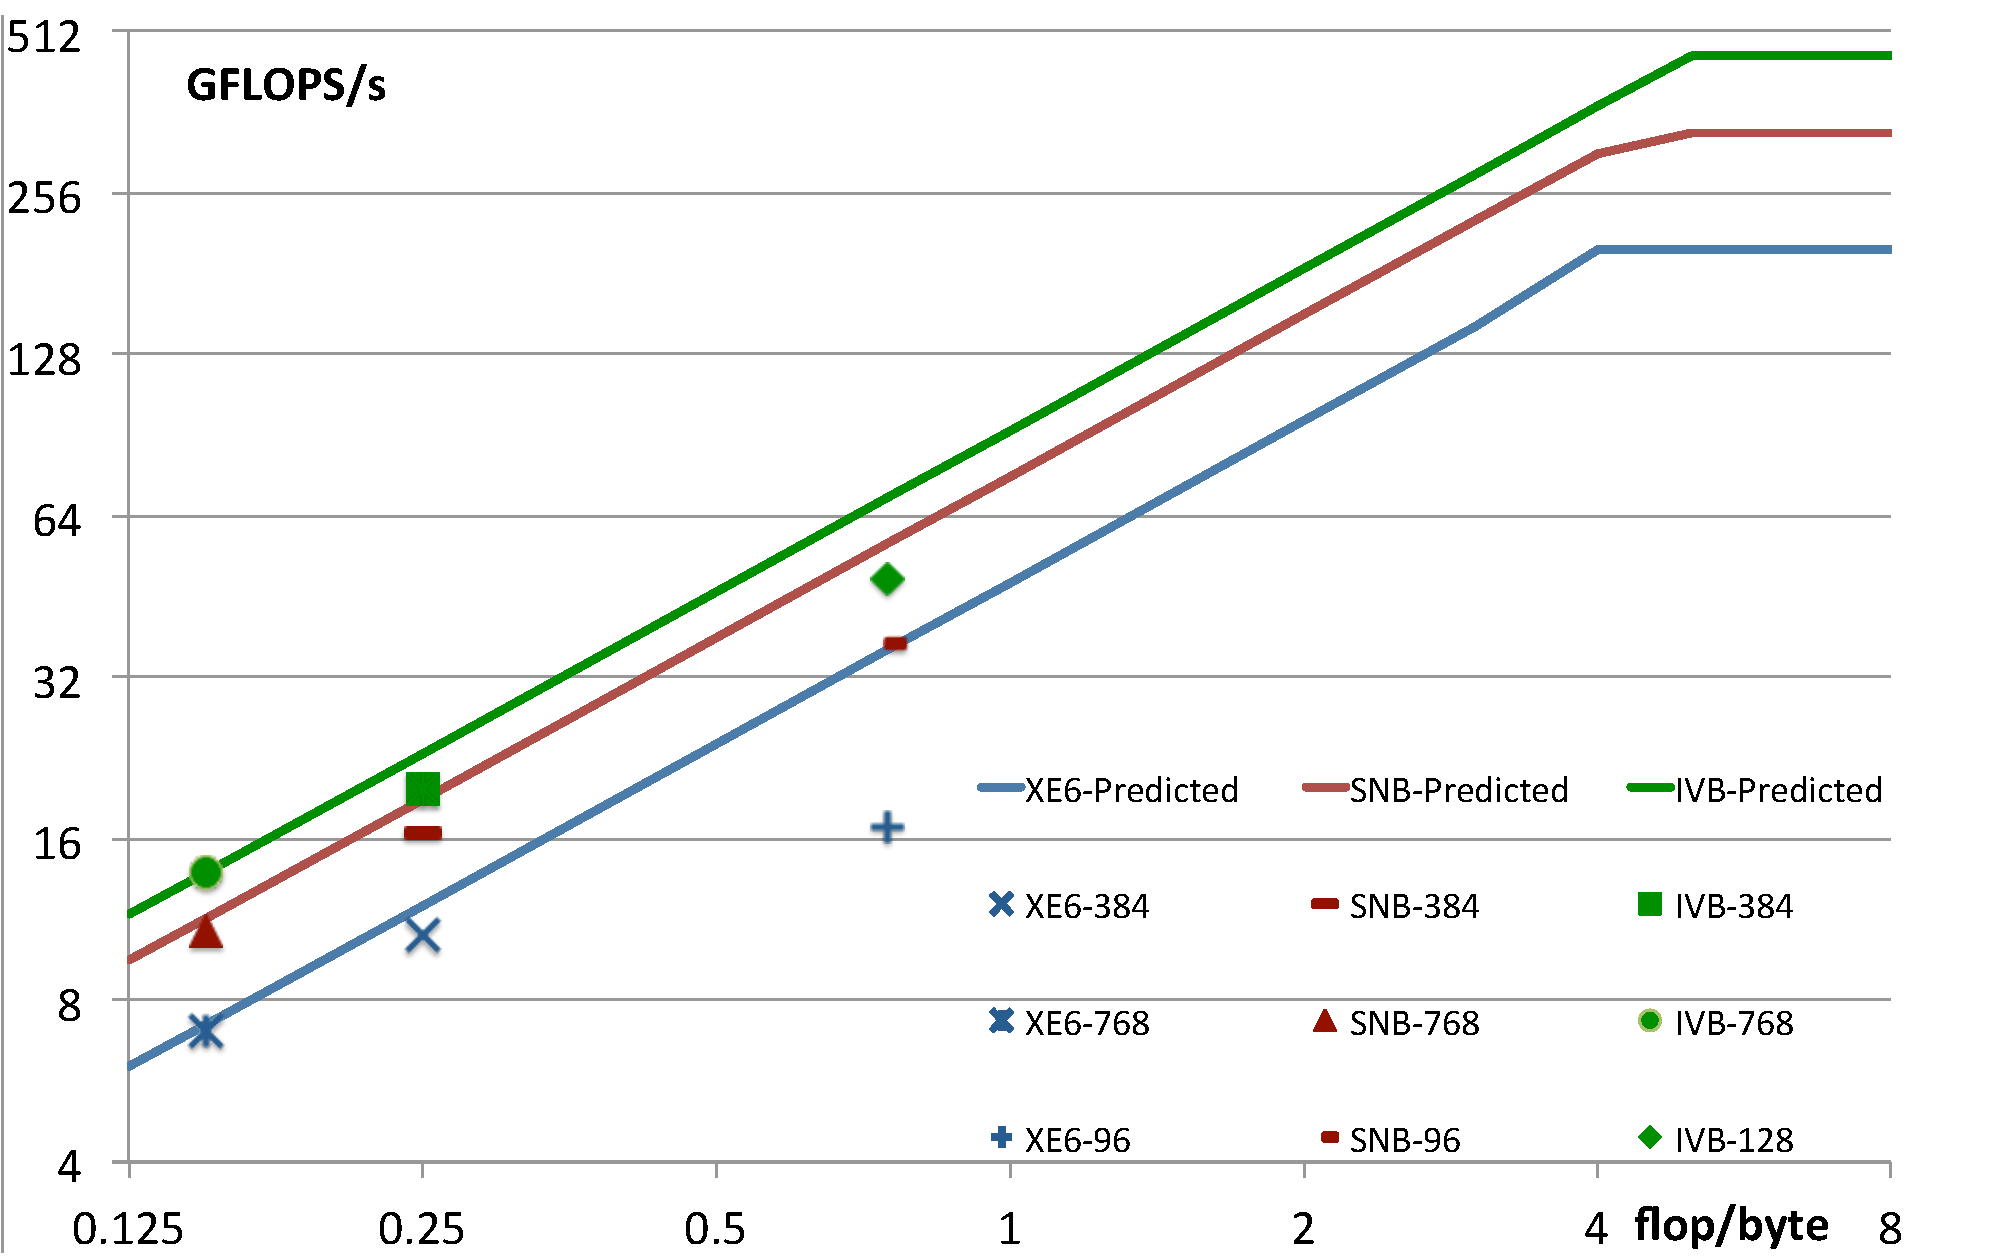
\includegraphics[width=0.99\textwidth]{jacobi_dram}
\caption{Performance validation for 3 different problem sizes corresponding to 3 flop/byte ratios. Since we included the communication, the larger problem size the less significant the communication overhead and thus the more accurate the prediction.}
\label{jacobi_dram}
\end{figure}

%We next reduced the problem size until it no longer fits in L3 cache and observed the best performance.
%In order to prevent data to be copied between L3 and DRAM, we shut off the communication.
%Figure~\ref{jacobi_l3} shows that the predicted performance correlates well with what we experimentally observed.

%\begin{figure}[htp]
%\centering
%\includegraphics[width=0.99\textwidth]{jacobi_l3}
%\caption{Performance validation for small problem sizes which fit in L3. The interprocess communication is shut off to eliminate the data transfer between DRAM and L3 within each time step}
%\label{jacobi_l3}
%\end{figure}


\subsection{HPGMG}
In this section we validate Exasat using HPGMG, a geometric multigrid framework for solving Helmholtz's equation in 3 dimensions.
This equation can be written in the form {\em Au = f}, where A is Helmholtz operator defined as follows.

\begin{equation}
a*alpha*u - b* \nabla \cdot (beta \nabla u)
\label{helmholtz}
\end{equation}

where, a and b are scalar constants, and alpha and beta are arrays of spatial coefficients.

HPGMG offers a V-cycle and a F-cycle solvers.
We use the former, which enables us to quickly estimate the overall performance by simply looking at the application behavior on a few fine grids only.
HPGMG consists of various stencil kernels.
For example, the red-black Gauss Seidel {\em smooth} kernel performs multiple consecutive red and black sweeps, which update grid data using neighboring values of the same grid; 
{\em residual} updates the residual grid using the right-hand-side and solution grids. 
These kernels are repeated at different levels of a V-cycle.

It is worth noting that more than 90\% of the application time is for running these 2 kernels on only the two finest grids.
As a result, in this report we show our analysis and validation of these 2 kernels on finest grids only. 


\subsubsection{XML description}
Figure~\ref{redblack} shows the source code of the red-black Gauss Seidel kernel.
It can be seen in the innest loop that the programmer fused the source code of the red and black phases using a stride-2 scheme. 
The programmer also simplified the update expression by using macros as shown in the code.
Exasat expands these macros and analyzes the final expression.
Fig.~\ref{redblackXML} shows the XML description of the red-black Gauss Seidel kernel.
One can easily recognize the arrays that this kernel references as well as the reference type (read/write) and the corresponding offsets.
The XML description also shows the number of different floating point operations used by the kernel.
This information is helpful in the case the cost of moving data does not dominate, e.g. when the problem size is small. 
Fig.~\ref{residual} shows the source code and the XML description of the residual kernel.


\begin{figure}[htp]
\begin{boxedverbatim}
      #define apply_op_ijk(x) 
      (
        -b*h2inv*(                                           \
          + beta_i[ijk+1      ]*( x[ijk+1      ] - x[ijk] )  \
          + beta_i[ijk        ]*( x[ijk-1      ] - x[ijk] )  \
          + beta_j[ijk+jStride]*( x[ijk+jStride] - x[ijk] )  \
          + beta_j[ijk        ]*( x[ijk-jStride] - x[ijk] )  \
          + beta_k[ijk+kStride]*( x[ijk+kStride] - x[ijk] )  \
          + beta_k[ijk        ]*( x[ijk-kStride] - x[ijk] )  \
        )
      )       
      #define calculate_Dinv()                               \
      (                                                      \
        1.0 / (a*alpha[ijk] - b*h2inv*(                      \
          + beta_i[ijk        ]*( valid[ijk-1      ] - 2.0 ) \
          + beta_j[ijk        ]*( valid[ijk-jStride] - 2.0 ) \
          + beta_k[ijk        ]*( valid[ijk-kStride] - 2.0 ) \
          + beta_i[ijk+1      ]*( valid[ijk+1      ] - 2.0 ) \
          + beta_j[ijk+jStride]*( valid[ijk+jStride] - 2.0 ) \
          + beta_k[ijk+kStride]*( valid[ijk+kStride] - 2.0 ) \
        ))                                                   \
      )
      for(k=klo;k<khi;k++){
        for(j=jlo;j<jhi;j++){
          for(i=ilo+((j^k^s^color000)&1)+1-ghosts;i<ihi;i+=2){ 
            int ijk=  i + j*jStride + k*kStride;
            double Ax     = apply_op_ijk(phi);
            double lambda = calculate_Dinv();
            phi[ijk] = phi[ijk] + lambda*(rhs[ijk]-Ax);
      }}}
\end{boxedverbatim}
\caption{Red-Black Gauss Seidel kernel, where {\em apply\_op\_ijk} and {\em calculate\_Dinv} are macros and will be expanded by the compiler of Exasat.}
\label{redblack}
\end{figure}


\begin{figure}[htp]
\begin{boxedverbatim}
<loop line="22" lvar="block" lb="0" ub="level->num_my_blocks" stride="1" 
adds="0" mults="0" divs="0">
<loop line="76" lvar="k" lb="klo" ub="khi" stride="1" adds="0" mults="0" divs="0">
<loop line="77" lvar="j" lb="jlo" ub="jhi" stride="1" adds="0" mults="0" divs="0">
<loop line="78" lvar="i" lb="ilo +((j ^ k ^ s ^ color000) & 1) + 1 - ghosts" 
ub="ihi" stride="2" adds="9" mults="5" divs="0">
<array name="rhs" component="" datatype="double" accesstype="readonly">
<access offset="(0 0 0 0 0 )" lvar="(  i j k)" reads="1" writes="0"/>
</array>
<array name="alpha" component="" datatype="double" accesstype="readonly">
<access offset="(0 0 0 0 0 )" dependentloopvar="(  i j k)" reads="2" writes="0"/>
</array>
<array name="beta_i" component="" datatype="double" accesstype="readonly">
<access offset="(0 0 0 0 0 )" lvar="(  i j k)" reads="2" writes="0"/>
<access offset="(1 0 0 0 0 )" lvar="(  i j k)" reads="2" writes="0"/>
</array>
<array name="beta_j" component="" datatype="double" accesstype="readonly">
<access offset="(0 0 0 0 0 )" lvar="(  i j k)" reads="2" writes="0"/>
<access offset="(0 1 0 0 0 )" lvar="(  i j k)" reads="2" writes="0"/>
</array>
<array name="beta_k" component="" datatype="double" accesstype="readonly">
<access offset="(0 0 0 0 0 )" lvar="(  i j k)" reads="2" writes="0"/>
<access offset="(0 0 1 0 0 )" lvar="(  i j k)" reads="2" writes="0"/>
</array>
<array name="valid" component="" datatype="double" accesstype="readonly">
<access offset="(1 0 0 0 0 )" lvar="(  i j k)" reads="2" writes="0"/>
<access offset="(0 1 0 0 0 )" lvar="(  i j k)" reads="2" writes="0"/>
<access offset="(0 0 1 0 0 )" lvar="(  i j k)" reads="2" writes="0"/>
<access offset="(-1 0 0 0 0 )" lvar="(  i j k)" reads="2" writes="0"/>
<access offset="(0 -1 0 0 0 )" lvar="(  i j k)" reads="2" writes="0"/>
<access offset="(0 0 -1 0 0 )" lvar="(  i j k)" reads="2" writes="0"/>
</array>
<array name="phi" component="" datatype="double" accesstype="readwrite">
<access offset="(0 0 0 0 0 )" lvar="(  i j k)" reads="14" writes="1"/>
<access offset="(1 0 0 0 0 )" lvar="(  i j k)" reads="1" writes="0"/>
<access offset="(0 1 0 0 0 )" lvar="(  i j k)" reads="1" writes="0"/>
<access offset="(0 0 1 0 0 )" lvar="(  i j k)" reads="1" writes="0"/>
<access offset="(-1 0 0 0 0 )" lvar="(  i j k)" reads="1" writes="0"/>
<access offset="(0 -1 0 0 0 )" lvar="(  i j k)" reads="1" writes="0"/>
<access offset="(0 0 -1 0 0 )" lvar="(  i j k)" reads="1" writes="0"/>
</array>
</loop>
</loop>
</loop>
</loop>
\end{boxedverbatim}
\caption{XML description of the Red Black Gauss Seidel smooth kernel (simplified).}
\label{redblackXML}
\end{figure}


\begin{figure}[htp]
\begin{boxedverbatim}
for(k=klo;k<khi;k++){
  for(j=jlo;j<jhi;j++){
    for(i=ilo;i<ihi;i++){
      int ijk = i + j*jStride + k*kStride;
      double Ax = apply_op_ijk(x);
      res[ijk] = rhs[ijk]-Ax;
}}}
<loop line="40" loopvar="k" lb="klo" ub="khi" stride="1" adds="0" mults="0">
<loop line="41" loopvar="j" lb="jlo" ub="jhi" stride="1" adds="0" mults="0">
<loop line="42" loopvar="i" lb="ilo" ub="ihi" stride="1" adds="19" mults="22">
<array name="x" component="" datatype="double" accesstype="readonly">
<access offset="(0 0 0 0 )" lvar="(  i j k)" reads="13" writes="0"/>
<access offset="(1 0 0 0 )" lvar="(  i j k)" reads="1" writes="0"/>
<access offset="(0 1 0 0 )" lvar="(  i j k)" reads="1" writes="0"/>
<access offset="(0 0 1 0 )" lvar="(  i j k)" reads="1" writes="0"/>
<access offset="(-1 0 0 0 )" lvar="(  i j k)" reads="1" writes="0"/>
<access offset="(0 -1 0 0 )" lvar="(  i j k)" reads="1" writes="0"/>
<access offset="(0 0 -1 0 )" lvar="(  i j k)" reads="1" writes="0"/>
</array>
<array name="rhs" component="" datatype="double" accesstype="readonly">
<access offset="(0 0 0 0 )" lvar="(  i j k)" reads="1" writes="0"/>
</array>
<array name="alpha" component="" datatype="double" accesstype="readonly">
<access offset="(0 0 0 0 )" lvar="(  i j k)" reads="1" writes="0"/>
</array>
<array name="beta_i" component="" datatype="double" accesstype="readonly">
<access offset="(0 0 0 0 )" lvar="(  i j k)" reads="1" writes="0"/>
<access offset="(1 0 0 0 )" lvar="(  i j k)" reads="1" writes="0"/>
</array>
<array name="beta_j" component="" datatype="double" accesstype="readonly">
<access offset="(0 0 0 0 )" lvar="(  i j k)" reads="1" writes="0"/>
<access offset="(0 1 0 0 )" lvar="(  i j k)" reads="1" writes="0"/>
</array>
<array name="beta_k" component="" datatype="double" accesstype="readonly">
<access offset="(0 0 0 0 )" lvar="(  i j k)" reads="1" writes="0"/>
<access offset="(0 0 1 0 )" lvar="(  i j k)" reads="1" writes="0"/>
</array>
<array name="valid" component="" datatype="double" accesstype="readonly">
<access offset="(1 0 0 0 )" lvar="(  i j k)" reads="1" writes="0"/>
<access offset="(0 1 0 0 )" lvar="(  i j k)" reads="1" writes="0"/>
<access offset="(0 0 1 0 )" lvar="(  i j k)" reads="1" writes="0"/>
<access offset="(-1 0 0 0 )" lvar="(  i j k)" reads="1" writes="0"/>
<access offset="(0 -1 0 0 )" lvar="(  i j k)" reads="1" writes="0"/>
<access offset="(0 0 -1 0 )" lvar="(  i j k)" reads="1" writes="0"/>
</array>
<array name="res" component="" datatype="double" accesstype="writeonly">
<access offset="(0 0 0 0 )" lvar="(  i j k)" reads="0" writes="1"/>
</array>
</loop>
</loop>
</loop>
\end{boxedverbatim}
\caption{The residual kernel and its corresponding XML description. The definition of the apply\_op\_ijk macro was shown earlier in Fig.\ref{redblack}.}
\label{residual}
\end{figure}


\subsubsection{Verifying the data working set}
While data is allocated in contiguous chunks, an update expression references to data elements of various arrays and in multiple dimensions. 
To avoid many accesses to high latency DRAM, portions of referenced arrays have to be fetched into cache before update operations can be carried on.
A set of such portions is commonly known as a {\em data working set}.
By examining the XML IR, the performance model can estimate the size of a working set. 
In addition, it can figure out the amount of data that we need to move between DRAM and cache as the working set slides.
First, considering problem sizes where the total amount of data is small enough to fit in DRAM and the data working set is small enough to fit in L3 cache.

The XML of red-black Gauss Seidel shows that this kernel updates new data to the {\em phi} array with offset (0, 0, 0).
The kernel also reads surrounding elements located in different arrays.
The data working set, therefore, contains 3 planes of {\em phi}, 2 planes of {\em valid}, 2 planes of {\em beta\_k}, 1 plane of {\em beta\_j}, {\em beta\_i}, {\em alpha}, and {\em rhs}. 
However, note that the kernel references consecutive planes of an array, allowing the compiler to cache recently used data for the next {\em data working set}.
Thus, Exasat can analyze the number of planes we need to fetch from DRAM for updating a plane of {\em phi}, ignoring the cache warming up time.
In particular, the XML description suggests that every plane update requires a new plane of {\em phi} to be fetched from DRAM (since the other 2 are already cached). 
The kernel also needs to fetch 1 plane from {\em valid}, {\em beta\_k}, {\em beta\_j}, {\em beta\_i}, {\em alpha}, and {\em rhs}.
Thus, at a grid level of a V-cycel, the total number of read planes is 7 and written planes is 1.

After the red-black Gauss Seidel is the residual.
Unlike the red-black Gauss Seidel kernel, the {\em residual} kernel updates data to the {\em res} array, which it does not read data from.
Thus, for every plane of {\em res}, we need to fetch a copy to cache to buffer the writing.  
The rest of the update expression of this kernel is similar to the red-black Gauss Seidel's.
Using the same analysis, we can find that the {\em data working set} of the residual contains 3 planes of x, 3 planes of valid, 2 planes of {\em res}, 2 planes of {\em beta\_k}, 1 plane of each {\em x}, {\em beta\_j}, {\em beta\_i}, and {\em rhs} arrays.
Also, the number of planes we need to move between L3 and DRAM in each plane update is 9, including 8 from reading and 1 from writing.

\begin{figure}[htp]
\centering
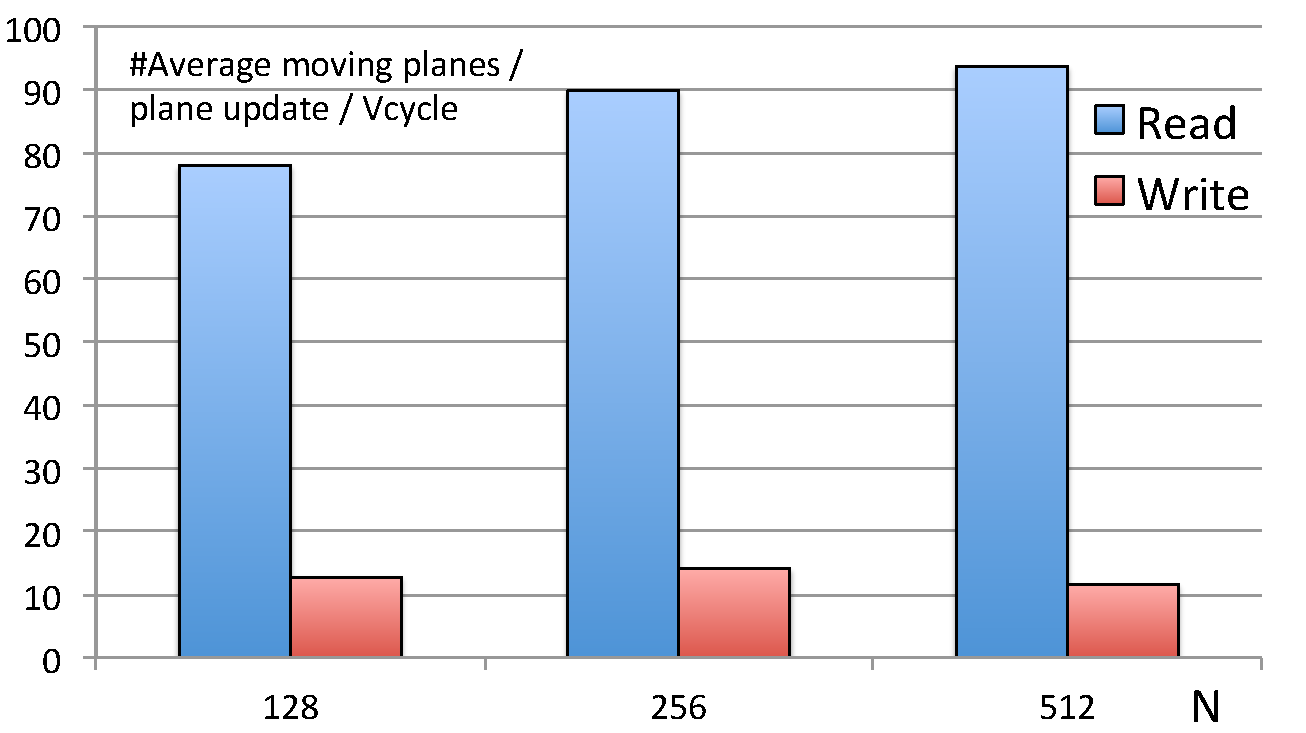
\includegraphics[width=0.99\textwidth]{hpgmg_dram}
\caption{The number of read and written planes measured via L3 misses and memory bandwidth.}
\label{hpgmg_dram}
\end{figure}

To verify our estimation on the {\em data working set}, we use a profiling tool to measure the amount of data transfer between DRAM and L3.
Although we would like to verify our estimation at the finest resolution (i.e. every single sweep), profiling tools introduce overheads.
As a result, we performed experimental validation at the granularity of a V-Cycle.
Fig.~\ref{hpgmg_dram} shows the average number of planes that we need to read and write per plane update.
In order to predict this information, one needs to know how often these 2 kernels are invoked.
Since Exasat keeps track of function calls and loops, we can extract this information.
In HPGMG, we found that each V-Cycle contains 8 red/black sweeps and 2 calls to residual.
Thus, in average, a plane update at the finest level requires 8 * 7 + 2 * 9 = 74 planes for read and 8 *1 + 2 * 1= 10 planes for write. 
At the next level, the size of the mesh is reduced by a factor of 8.
Thus, for the 3 finest levels we need an average of 74 * (1 +1 /8 + 1/64)= 84.4 planes for read and 10 * (1 + 1/8 + 1/64) = 11.4 planes for write.
However, if the problem size is small (e.g. with $128^3$) the second and third levels fit in L3 and the number of reads is negligible.
Thus, the number of read planes in such cases is 74.
It can be seen in Fig.~\ref{hpgmg_dram} that the profiling results support our analysis. 

We then ran and collected the total running time of HPGMG on different node architectures.
Fig.~\ref{hpgmg_overall} shows the measured and predicted executime times. 
We found that the prediction was relatively accurate, especially on SNB and IVB.
When we excluded the communication overheads, the performance difference was even smaller.
The remaining discrepancy was because of errors in calibrating memory bandwidth and other unaccounted activities such as restriction and interpolation.

\begin{figure}[htp]
\centering
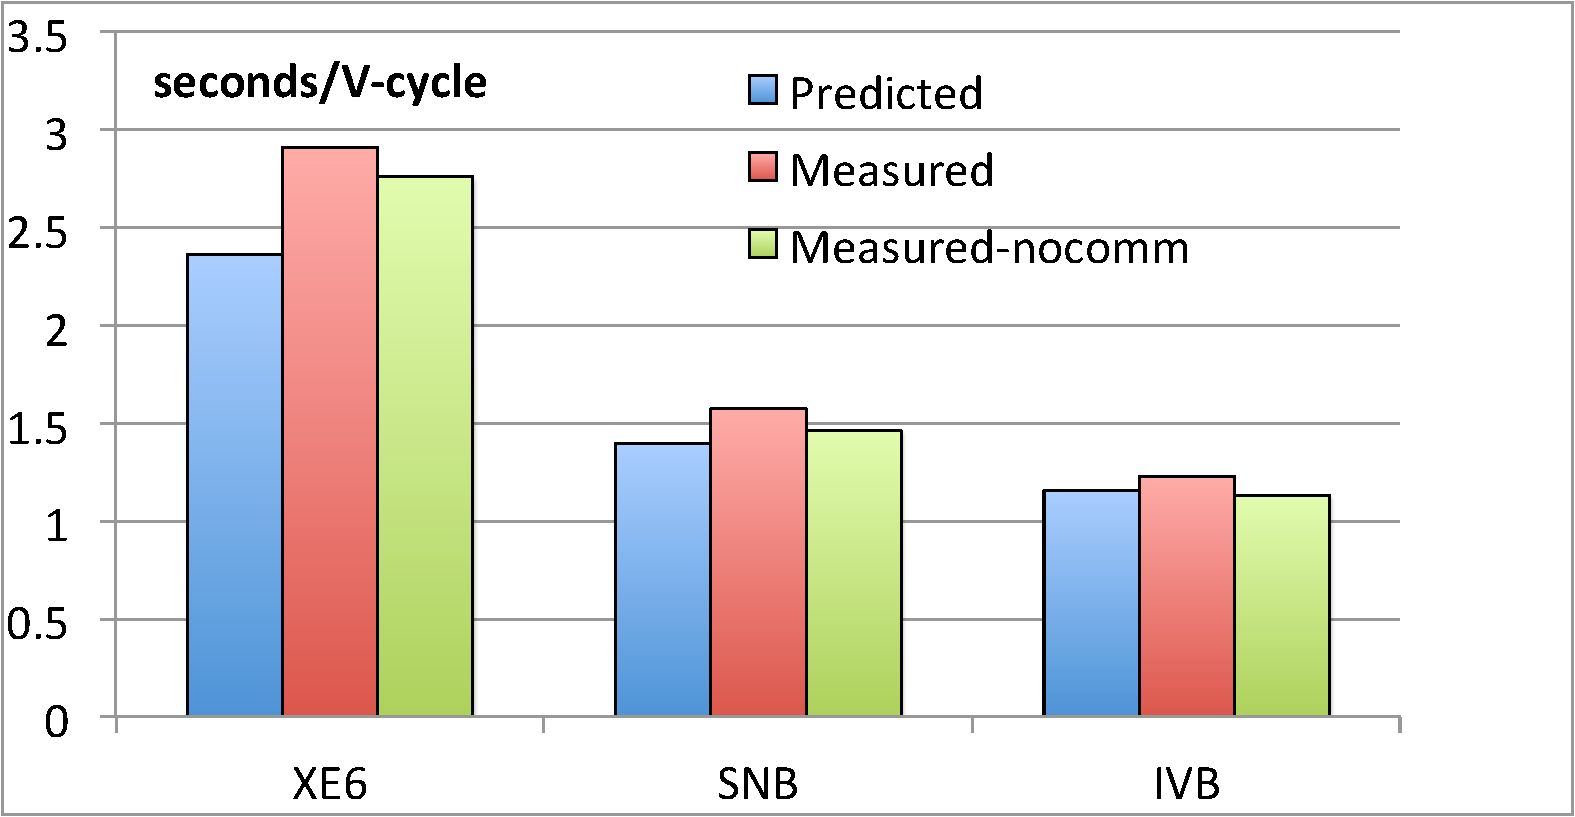
\includegraphics[width=0.99\textwidth]{hpgmg_overall}
\caption{Predicting the performance of HPGMG.}
\label{hpgmg_overall}
\end{figure}


\section{Limitations}

\subsection{Compiler}
Exasat is a static analysis framework.
Thus, it can't resolve or completely resolve a few language constructs due to lack of runtime information. 

\subsubsection{Resolving aliases}
In C, C++, and Fortran, the programmer can reference arrays via pointers.
Unless the programmer explicitly describes whether the targeted arrays do not overlap (e.g. using the {\em \_restrict} keyword), a compiler generally cannot reason about this information. 
This limitation also applies to Exasat.
In particular, if it is not clear whether 2 targeted arrays overlap, Exasat has to conservatively assume that they are separate ones \footnote{a generic compiler may assume differently that arrays overlap by default}.
The consequence is that the predicted demand on memory bandwidth is higher than the actual one if the assumption is not correct.
We are implementing alias analysis so Exasat can figure out if 2 pointers point to the same array in some situations.

\subsubsection{Resolving function pointer}
Function pointer is often used in C to allow the programmer to quickly select an implementation of a routine among many available options.
In this case, the value of a function pointer is often input dependent, disallowing a compiler to reason about its value at static time.
Function pointer is also used to implement function callbacks, which allows the parameter list of a function to contain another function.
In this case, a function name is passed to a function call as an argument.
If this argument is not input dependent, Exasat is able to analyze the calling chain. 


\subsubsection{Branch prediction}
Predicting whether a branch will be taken or not taken is a challenging task.
Generally a compiler has to defer such decision until the branch instruction is about to execute.
We plan to take an instrumentation approach, where we automatically insert profiling code into the source code.
By running the resulting program for particular input sets, we can collect relatively accurate branching information.

\subsection{Performance model}
The performance model currently cannot handle some array access patterns such as gather and scatter.
In addition, it ignores interprocess communication, though the XML description contains information of communication.
As a result, the estimated performance of the overall application may differ significantly from the measured one if these activities account for a major part of the application running time.

\section{Conclusion}
In this report, we have presented new capabilities in Exasat to handle various array access styles and predict the memory bandwidth demand of the application on the memory subsystem.
Specifically, we showed how the compiler of Exasat generated user-readable XML representation of stencil kernels in single-grid and multigrid solvers.
We then explained how the performance model of Exasat predicted the performance behavior of an application given the corresponding XML description and hardware specifications.
Finally we conducted experiments on various hardware architectures to validate the analysis.
In particular, we collected hardware specifications such as memory bandwidth and peak computation rate.
In addition, we used PAPI, a profiling tool to measure the amount of data transferred between DRAM and L3.
Experimental results demonstrated that, for most typical problem sizes,  the prediction error is always less than 20\%.  %when counting communication overheads. 
We found that the discrepancy is mostly due to the communication overheads that the performance model currently ignores (the accuracy rate would be more than 90\% without communication).
This problem will be lifted in the future when we take communication into account. 
Nevertheless, the most important contribution of Exasat is that with the tool we were able to correctly capture the performance behavior of the application when the problem size and/or hardware specification vary.

In the future, we plan to extend the compiler of Exasat so it can handle more memory access patterns, including those not in the stencil class.
In addition, we will extend the performance model to support many-core architectures, which offers higher computing rate as well as memory bandwidth but come with more complicated interconnections among processor cores/sockets.

\bibliography{exasat}{}
\bibliographystyle{plain}

\end{document}
